\subsection{Simulation}

To verify the validity of the \textbf{PD} controller for this task, simulations were run in MATLAB. The simulation set the motors to a common speed, so that the controller always makes the robot move forward when $\theta=0$ and lower the speed of a motor on one side to turn. This is the same way as the controller is implemented on the robot. Both motors speed can therefore be set into one variable that is defined as the difference between the motor speeds ($\Delta v = v_L-v_R$). \\
\indent The simulation used a sinusoid as input to the controller, simulating that the robot travelled along a line that consistently turn from left to right and back again. The results can be seen in Fig. \ref{fig:sim_t_error} and \ref{fig:sim_LR_motor}

\begin{figure}[H]
    \centering
    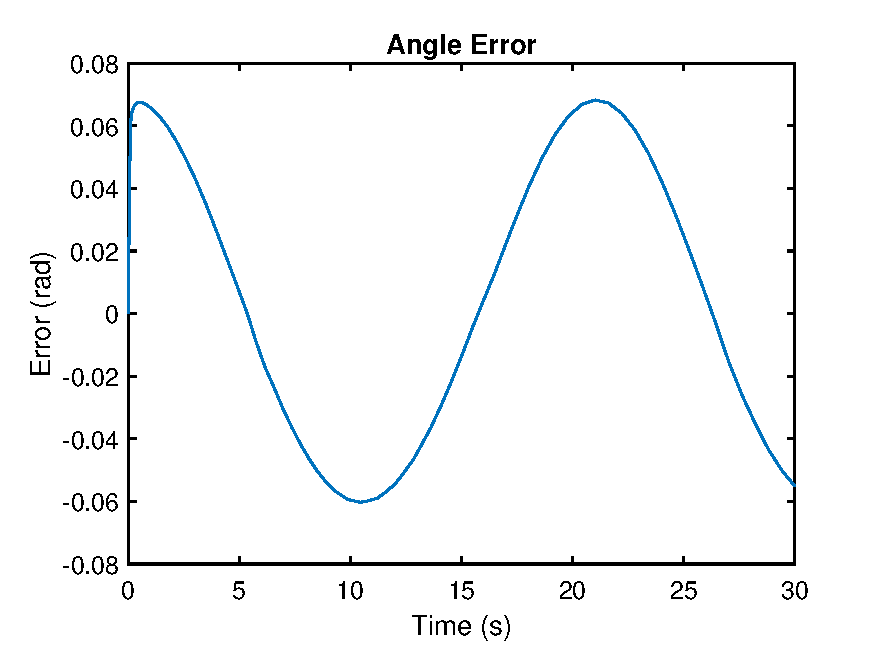
\includegraphics[width=0.7\textwidth]{img/theta_error.eps}
    \caption{The error between the robots pose and the line.}
    \label{fig:sim_t_error}
\end{figure}

\begin{figure}[H]
    \centering
    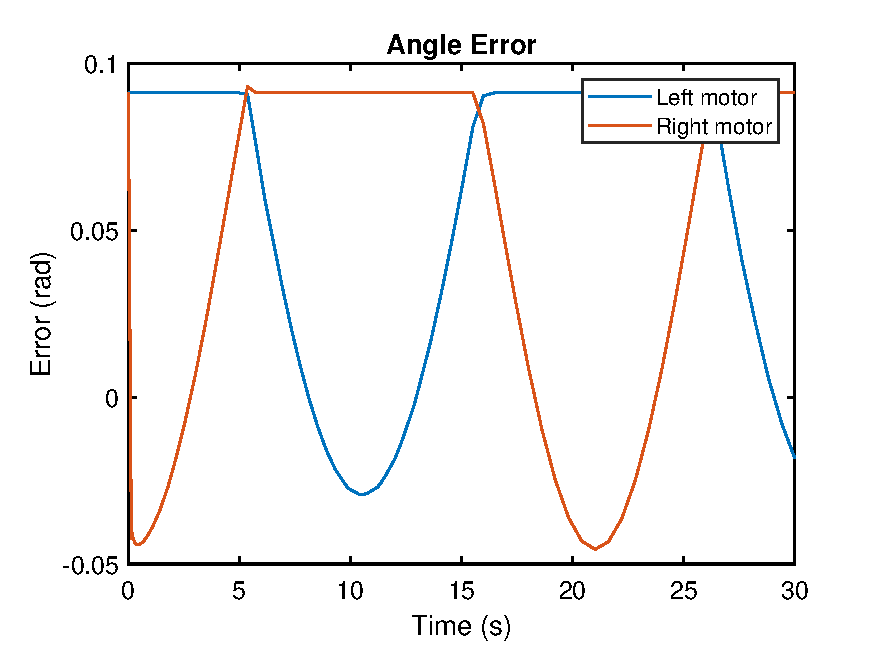
\includegraphics[width=0.7\textwidth]{img/LR_motors.eps}
    \caption{The motor output for the results in Fig.\ref{fig:sim_t_error}.}
    \label{fig:sim_LR_motor}
\end{figure}

The results presented above is evidence that a \textbf{PD} controller can be used for a line follower. 
